\documentclass{article}

\usepackage{times}
\usepackage{graphicx} % more modern
\usepackage{subfigure} 
\usepackage{natbib}
\usepackage{algorithm, algorithmic}
\usepackage{hyperref}
\usepackage{amssymb, mathtools}
\usepackage{xcolor,colortbl}
\newcommand{\theHalgorithm}{\arabic{algorithm}}


% Employ the following version of the ``usepackage'' statement for
% submitting the draft version of the paper for review.  This will set
% the note in the first column to ``Under review.  Do not distribute.''
\usepackage{icml2016} 

% Employ this version of the ``usepackage'' statement after the paper has
% been accepted, when creating the final version.  This will set the
% note in the first column to ``Proceedings of the...''
%\usepackage[accepted]{icml2016}


% The \icmltitle you define below is probably too long as a header.
% Therefore, a short form for the running title is supplied here:
\icmltitlerunning{Globally Induced Forest}

% ============================== PATHS =================================== %
\graphicspath{{./images/}}
% ============================== COLORS =================================== %
\definecolor{orange}{HTML}{FFA500}
\definecolor{dodgerblue}{HTML}{1E90FF}
\definecolor{deepgreen}{HTML}{0AF191}
\definecolor{purplish}{HTML}{E21173}

% ============================== COMMANDS =================================== %
\DeclareMathOperator*{\argmin}{arg\,min}
\DeclareMathOperator*{\argmax}{arg\,max}


\newcommand{\best}{\cellcolor{lightgray}}
\newcommand{\bestA}{\cellcolor{orange}}
\newcommand{\bestB}{\cellcolor{dodgerblue}}


\begin{document} 

\twocolumn[
\icmltitle{Globally Induced Forest: A Prepruning Compression Scheme}

% It is OKAY to include author information, even for blind
% submissions: the style file will automatically remove it for you
% unless you've provided the [accepted] option to the icml2016
% package.
\icmlauthor{Jean-Michel Begon}{jm.begon@ulg.ac.be}

\icmlauthor{Arnaud Joly}{a.joly@ulg.ac.be}
\icmlauthor{Pierre Geurts}{p.geurts@ulg.ac.be}
\icmladdress{Department of Electrical Engineering and Computer Science
University of Liège \\
Institut Montefiore, Sart Tilman B28, B-4000 Liège, Belgium}
% You may provide any keywords that you 
% find helpful for describing your paper; these are used to populate 
% the "keywords" metadata in the PDF but will not be shown in the document
\icmlkeywords{Decision tree, Random forest, Extremely randomized trees, 
pruning, node budget, memory constraint, compression, growing algorithm, greedy 
selection}

\vskip 0.3in
]

\begin{abstract} 
Tree-based ensemble models are heavy memory-wise. An undesired state of affairs 
considering nowadays datasets, memory-constrained environment and 
fitting/prediction times.
In this paper, we propose the Globally Induced Forest (GIF) to remedy this 
problem. GIF is a fast prepruning approach to build lightweight ensembles by 
iteratively deepening the current forest. It mixes local and global 
optimizations to produce accurate predictions under memory constraints in 
reasonable time.
We show that the proposed method is more than competitive with standard 
tree-based ensembles under corresponding constraints, and can sometimes even 
surpass much larger models. 
\end{abstract} 

\section{Introduction}
\label{sec:introduction}

Decision forests, such as Random Forest \cite{breiman2001random} and Extremely 
Randomized Trees \cite{extratrees}, are popular methods in the machine 
learning community. This popularity is due to their overall good accuracy, 
relative ease-of-use, short learning/prediction time and interpretability. The 
good accuracies are a consequence of the variance reduction through the 
ensemble averaging. The ease-of-use is due to the small number of 
well-understood hyper-parameters. In particular, the accuracy is a monotonic 
increasing function of the number of trees.
%and the deeper the tree, the better the variance reduction. 
The computational efficiency in the learning phase originates in the greedy 
building mechanism whereas it is a consequence of the partitioning tree 
structure during the prediction phase. Finally, the model is interpretable in 
the sense that it yields, as a by product, a measure of variable importances 
with respect to the goal.

Over the past decade, datasets have become bigger and bigger. The number of 
instances $N$ has increased and the community has turned to very 
high-dimensional learning problems. The former has led to bigger trees, as the 
number of nodes in a tree is $O(N)$. The latter, on the other hand, tends to 
steer toward larger forests. Indeed, the variance of individual trees tends to 
increase with the dimensionality $P$ of the problem \cite{l1basedcomp}. 
Therefore, the adequate number of trees $T$ increases with the dimensionality. 
Overall, this change of focus might render tree-based ensemble techniques 
impractical memory-wise, as the total footprint is $O(N \times T(P))$. 

Aside from big data, other areas of machine learning suffer from the high 
memory demand of tree-based methods. For instance, low-memory devices, such as 
mobile phones and embedded systems, require lightweight models. In addition, 
bigger is not always better when it comes to tree-based ensembles.
If it true that the more trees, the better the model, this is not the case for 
deeper individual trees.
Smaller models also implies faster predictions, dear to real-time applications.
%Cite kinect?

All in all, tree-based models might benefit from lighter memory footprint in 
many different ways.


\section{Related work}
\label{sec:relatedWork}
Memory constraints of tree-based ensemble methods is not a new topic and has 
been tackled from various perspectives, which can be partitioned into 
tree-agnostic and tree-aware methods.

The former set of techniques are general purpose methods which can deal with  
any ensembles. We can distinguish further between re-learning algorithms ({\it 
e.g.} \citet{domingos1997oracle}, \citet{menke2009oracle}), which try to come 
up with a smaller, equivalent models, and ensemble pruning methods. Those try 
to eliminate some of the redundant base learners constituting the ensemble (for 
a review of those methods, please consult \citet{tsoumakas2008enspruning}, 
\citet{rokach2016enspruning}). 
%Why don't we compare to them?

Tree-aware methods strive to build smaller trees by limiting the total number 
of nodes within the forest. They either work with a subsample of the training 
set ({\it e.g.} \citet{breiman1999pasting}), or on the whole learning set. The 
latter can be partitioned into pre- and post-pruning families. 
Pre-pruning methods aim at stopping the development of uninteresting branches 
in the top down induction procedure. On the other hand, the post-pruning 
methods's goal is to discard {\it a posteriori} branches which do not provide 
significant accuracy improvements.

Originally, the idea was introduced to control the model complexity and avoid 
overfitting. The advent of ensemble methods somewhat cast aside those 
techniques as the averaging mechanism became responsible for reducing the 
learning algorithm's variance. Nonetheless, a few ensemble-wise, post-pruning 
methods have recently emerged with a focus on memory minimization. In both 
\citet{meinshausen2009forestgarrote} and \citet{l1basedcomp}, the compression 
is formulated as a slightly different global constrained optimization problem. 
In opposition, compression is undertook by a sequential optimization problem in 
\citet{ren2015glorefinement}.
In \citet{vleeschouwer2015mitimemreq}, the authors alleviate the leaves' memory 
requirements by clustering their conditional distributions. After computing a 
wavelet coefficient for each node, the authors of \citet{elisha2016wavelet} 
discard all the nodes which are not on the path to a node of sufficient 
coefficient.
All these methods are able to retain almost the full forest accuracies while 
offering a significant memory improvement, leaving their requirement for 
building the whole forest first, and consequently the high temporary memory and 
computational costs, as their only major drawbacks.


\paragraph{Contribution and outline}
In this paper, we propose the Globally Induced Forest (GIF), an algorithm 
which, under a node budget constraint, iteratively and greedily deepens the 
trees by optimizing globally the sequence of nodes to develop and their 
associated weights, while still choosing locally, based on the standard score 
criterion, the splitting variables and cut points at all tree nodes. 

This mix of global, local and greedy optimization results in a fast pre-pruning 
approach to build lightweight, yet accurate forests learned on the whole 
training set. Contrary to post-pruning approaches, GIFs circumvent the need to 
build the whole forest first, resulting in a fast learning algorithm and 
discarding the need for a large temporary storage.

In section \ref{sec:gif}, we introduce the GIF algorithm and how it can be 
applied for both regression (subsection \ref{subsec:regression}) and 
classification (subsection \ref{subsec:classification}). 
In section \ref{sec:analysis}, we show that our proposed algorithm, with its 
default set of parameters, perform well on many datasets, even surpassing much 
larger models sometimes. We then conduct an analysis of the hyper-parameters 
entailed in GIF (subsection \ref{subsec:hyperparams}). Since GIF shares some 
resemblance to Boosting, the two are compared in subsection 
\ref{subsec:boosting}, before concluding and outlying future works in section 
\ref{sec:conclusion}. 


\section{Globally Induced Forest}
\label{sec:gif}

GIFs rely on the view of the forest as a linear model in the ``forest space'', 
a binary $M$-dimensional space, where $M$ is the total number of nodes in the 
whole forest \cite{l1basedcomp}:

\begin{equation}\label{eq:fs}
\vspace{-1em}
\hat{y}(x) =  \frac{1}{T} \sum_{j=1}^{M} w_j z_j(x),
\end{equation}

where the indicator function $z_j(x)$ is $1$ if $x$ reaches node $j$
and $0$ otherwise, and $w_j$ is the prediction at a node $j$ if $j$ is
a leaf and $0$ otherwise. In regression, $w_j \in \mathbb{R}$ would be the 
average value of the subset of outputs reaching node $j$. In classification, 
$w_j \in \mathbb{R}^K$ is a vector of dimension $K$, where $w_j^{(k)}$ 
($k=1,\ldots,K$) is the probability associated to class $k$.



%http://ctan.mackichan.com/macros/latex/contrib/algorithms/algorithms.pdf
%http://tex.stackexchange.com/questions/261859/how-to-put-a-line-number-with-levels-in-algorithm
\begin{algorithm}[tb]
   \caption{Globally Induced Forest}
   \label{alg:gif}
\begin{algorithmic}[1]
    \STATE {\bfseries Input:} $D= (x_i,y_i)_{i=1}^N$, the learning set; ${\cal 
    A}$, the tree learning algorithm; $L$, the loss function;  $B$, the node 
    budget; $T$, the number of trees; $CW$, the candidate window size; 
    $\lambda$, the learning rate.
    \STATE {\bfseries Output:} An ensemble $S$ of $B$ tree nodes with their 
    corresponding weights.
    \STATE {\bfseries Algorithm:}
    \STATE $S=\emptyset$; $C=\emptyset$; $t=1$
    \STATE $\hat{y}^{(0)}(.)= \argmin_{y \in \mathbb{R}^K} \sum_{i=1}^{N} 
    L(y_i, 0)$
    \STATE Grow $T$ stumps with ${\cal A}$ on $D$ and add the left and right 
    successors of all stumps to  $C$.    
    \REPEAT
        \STATE $C_t$ is a subset of size $\min\{CW, |C|\}$ of $C$ chosen 
        uniformly at random.
        \STATE Compute:
            \vspace{-1.5em}
            \begin{equation*}
            (j^*,w^*_j)=\argmin_{j\in C_t, w\in \mathbb{R}^K} 
            \sum_{i=1}^{N} L \left(y_i, \hat{y}^{(t-1)}(x_i) + w z_j(x_i) 
            \right)
            \end{equation*}
            \vspace{-1em}
        \STATE $S=S\cup\{(j^*,w^*_j)\}$; $C=C\setminus\{j^*\}$; \\
            $y^{(t)}(.)=y^{(t-1)}(.)+\lambda w^*_{j^*} z_{j^*}(.)$
        \STATE Split $j^*$ using ${\cal A}$ to obtain children $j_l$ and $j_r$
        \STATE $C=C\cup\{j_l,j_r\}$; $t++$
    \UNTIL{budget $B$ is met}
\end{algorithmic}
\end{algorithm}

%TODO node count ?

GIF's learning phase is described in Algorithm \ref{alg:gif}.
Starting from a constant model (step 5), it builds an additive model in the 
form of Equation (\ref{eq:fs}) by incrementally adding new node indicator 
functions in a stagewise fashion in order to grow the forest.
At each step, a subset of candidate nodes $C_t$ is built uniformly at random 
from the total candidate list $C$ (step 8). The node $j^*$ among those of $C_t$ 
which contributes the most to a decrease of the global loss is selected (step 
9) and introduced in the model via its indicator function $z_{j^*}$ and its 
optimal weight $w^*_j$ tempered by some learning rate $\lambda$ (step 10). This 
node is then split locally according to the reference tree growing strategy 
$\mathcal{A}$ (step 11) and replaced by its two children in the candidate list 
(step 12). The process is stopped when the node budget $B$ is reached. 

The predictions follows from Equation (\ref{eq:fs}) with the slight difference 
that 
internal nodes now have a weight as well. This could trivially be gotten rid of 
by pushing all the weights to the leaves.


Note that GIF is very similar to a least-square boosting algorithm
\cite{hastie2009}, where the set of base learners would be composed of
node indicator functions and would be expanded at each iteration.

\paragraph{Node selection and weight optimization}
Step 9 of Algorithm \ref{alg:gif} can be decomposed into two parts. Firstly, 
the optimal weight for a given candidate node is computed. Then, the optimal 
node---the one which reduces the loss the most---is selected with 
exhaustive search. Also note that computing the error can be done efficiently 
by going only over the instances reaching node $j^*$:

\begin{align}\label{eq:nodeSel}
w_j^{(t)} &= \argmin_{w \in \mathbb{R}^K} \sum_{i=1}^{N} L \left(y_i, 
\hat{y}^{(t-1)}(x_i) + w z_j(x_i)  \right) \\
\text{err}_j^{(t)} &= \sum_{i=1}^{N} L \left(y_i, \hat{y}^{(t-1)}(x_i) + 
w_j^{(t)} z_j(x_i)  \right) \\
j_t^* &= \argmin_{j \in C_t} \text{err}_j^{(t)} = \argmax_{j \in C_t} 
\text{err}^{(t-1)} - \text{err}_j^{(t)} \\
\text{gap}_j^{(t)} &= \text{err}^{(t-1)} - \text{err}_j^{(t)} \\
&= \sum_{i=1}^{N} \left[ L\left(y_i, \hat{y}^{(t-1)}(x_i)\right) - L\left(y_i, 
\hat{y}^{(t)}(x_i)\right) \right] \\
%&= \sum_{i\in Z_j} \left[ L\left(y_i, \hat{y}^{(t-1)}\right) - L\left(y_i, 
%\hat{y}^{(t)}\right) \right] + \sum_{i\notin Z_j} \left[ L\left(y_i, 
%\hat{y}^{(t-1)}\right) - L\left(y_i, \hat{y}^{(t)}\right) \right]  \\
%&= \sum_{i\in Z_j} \left[ L\left(y_i, \hat{y}^{(t-1)}\right) - L\left(y_i, 
%\hat{y}^{(t)}\right) \right] + \sum_{i\notin Z_j} \left[ L\left(y_i, 
%\hat{y}^{(t-1)}\right) - L\left(y_i, \hat{y}^{(t-1)}\right) \right]  \\
&= \sum_{i\in Z_j} \left[ L\left(y_i, \hat{y}^{(t-1)}(x_i)\right) - L\left(y_i, 
\hat{y}^{(t)}(x_i)\right) \right]
\end{align}

since $\hat{y}^{(t-1)}(x_i) \neq \hat{y}^{(t)}(x_i)$ only for the instances 
reaching node $j$: $i \in Z_j$. Due to the partitioning property of the tree, 
it means that, at each iteration, computing the optimal weights for all the 
nodes of a given tree is at most $O(N)$, assuming a single weight optimization 
runs in linear time in the number of instances reaching that node.

\paragraph{Tree learning algorithm}
The tree learning algorithm is responsible for splitting the data reaching a 
node. This choice is made locally, meaning that it disregards the current 
predictions of the model. In order to encourage diversity among candidates, we 
have chosen to use the Extremely randomized trees's splitting rule 
\cite{extratrees}: $m$ out of $p$ features are selected uniformly at random 
and, for each feature, a cut point is chosen uniformly at random between the 
current minimum and maximum value of this feature. The final decision function 
is the one which reduces the impurity score---variance in regression, gini 
index in classification---the most.

\paragraph{Node budget}
The node budget accounts for the total number of nodes in the resulting forest. 
That is, both internal (splitting) and external (decision) nodes. The root 
nodes are only accounted for when one of its children is taken into the model.

\paragraph{Forest's shape}
Three parameters interact to influence the forest's shape: the number of trees 
$T$, the candidate window size $CW$ and the learning rate $\lambda$. 

On the one hand, $CW=1$ means that the forest's shape is predetermined and 
solely governed by the number of trees. Few trees impose a development in 
depth, while many trees encourages in-breadth growth. Since the selection 
is uniform over the candidates, it also implies that well developed trees are 
more likely to get developed again, as choosing a node means replacing it in 
the candidate list by its two children (unless it is a leaf). This aggregation 
effect should somewhat be slowed when increasing the number of trees 
(in-breadth development).

On the other hand, $CW=+\infty$ means that the algorithm takes the 
time to optimize completely the node it chooses, giving it full rein to adapt 
the forest's shape to the problem at hand. In that case, the learning rate 
plays an important role (Figure \ref{fig:LRShape}). If it is low, the node will 
not be well optimized and the learning algorithm will look for similar nodes. 
In opposition, if the learning rate is high, the node will be well optimized 
and the algorithm will turn to different nodes.
As similar nodes tend to be located roughly at the same place in trees, low 
(resp. high) learning rate will encourage in breadth (resp. in depth) 
development.

\paragraph{Regularization}
The learning rate is the most explicit regularization parameter. However, many 
other factors act as implicit regularization in GIF, allowing at the same time 
for faster learning. 
Namely, the local splitting done by the tree learning algorithm $\mathcal{A}$, 
the greedy, stagewise weight optimization and the candidate subsampling.


\paragraph{GIF versus Boosting}
From a conceptual point of view, GIF is somewhat an intermediate model 
between Random forest and Boosting. Similarly to Boosting, the additive model 
is  built sequentially by optimizing globally some weight. Contrary to 
Boosting, the trees' splits in GIF are not optimized globally and no depth 
restriction is imposed on the trees constituting the ensemble. Notice also that 
the weight can be multidimensional, whereas it is usually scalar in Boosting.


\subsection{Regression}
\label{subsec:regression}

Under the $L2$-norm, the optimization (\ref{eq:nodeSel}) becomes:

\begin{align}\label{eq:L2min}
w_j^{(t)} &=  \argmin_{w \in \mathbb{R}} \sum_{i \in Z_j} \left(r_i^{(t-1)} - 
w\right)^2
\end{align}

where $r_i^{(t-1)} = y_i - \hat{y}^{(t-1)}(x_i)$ is the residual at time $t-1$.
The optimal weight is the average residual:

\begin{align}\label{eq:L2Solution}
w_j^{(t)} = \frac{1}{|Z_j|} \sum_{i \in Z_j} r_i^{(t-1)}
\end{align}

In the case of a unit learning rate and a single tree, the model's prediction 
coincide with the ones the underlying tree would provide (see Appendix 
\ref{app:Equiv}).

Extending to the multi-output case is straightforward: one only needs to fit a 
weight independently for each output. The loss becomes the sum of the 
individual losses over each output.

\subsection{Classification}
\label{subsec:classification}

Binary classification can either be tackled with the square loss, recasting the 
classes as $\{-1, +1\}$, or by employing a more suited loss function. Indeed, 
the former has the disadvantage that it will penalize correct classification if 
the prediction overshoots the real value.

In multiclass classification, one has several options. A first possibility is 
to build several binary classification models using a binary loss function. 
Interestingly, this can be done in a single learning phase by attributing one 
output per model. In contrast with a pure one-versus-one or one-versus-rest 
technique, the individual models would not be independent as they share the 
same forest structure.

A second approach is to employ a custom multiclass loss. An example of such a 
loss function is the multiclass exponential loss discussed in 
\citet{zhu2009multiadaboost}. Firstly, we must encode the class into a 
$K$-dimensional vector so that


\begin{align}\label{eq:MEencode}
y_i^{(k)} = \begin{cases}
1, &\text{ if the class of } y_i \text{ is } k \\
-\frac{1}{K-1}, &\text{otherwise}
\end{cases}
\end{align}

This representation agrees with the binary case and is less demanding than a 
one-versus-rest approach: the negative classes weigh the same as the correct 
one; $\sum_{k=1}^{K} y_i^{(k)} = 0$.

With this representation, the optimization problem (\ref{eq:nodeSel}) becomes:

\begin{align}\label{eq:MEmin}
w_j^{(t)} &=  \argmin_{w \in \mathbb{R}^K} \sum_{i \in Z_j} \exp 
\left(\frac{-1}{K} y_i^T \left(\hat{y}^{(t-1)}(x_i) + w \right)\right)
\end{align}

This program is convex and verifies the following constraint at the optimum:

\begin{align}\label{eq:MEequation}
\alpha_j^{(t-1, k)}\phi^{(k)}(w) &= \alpha_j^{(t-1, l)}\phi^{(l)}(w) \quad i 
\leq k,l \leq K \\
\alpha_j^{(t-1, k)} &= \sum_{i \in Z_j^{(k)}} \exp \left( - \mu_i^{(t-1)} 
\right) \\
\mu_i^{(t-1)} &= \frac{1}{K} \sum_{k=1}^{K} y_i \hat{y}^{(t-1, k)}(x_i) \\
\phi^{(k)}(w) &= \exp \left( - \frac{1}{K} \psi^{(k)}(w) \right) \\
\psi^{(k)}(w) &= -w^{(k)} + \frac{1}{K-1} \sum_{l=1, l\neq k}^{K}  w^{(l)}
\end{align}

where $Z_j^{(k)} = \{1 \leq i \leq N | z_{i,j} = 1 \wedge y_i^{(k)} = 1 \}$ is 
the subset of learning instances of class $k$ reaching node $j$. In words, 
$\mu_i^{(t-1)}$ is the hyper-margin of instance $i$ at time $t-1$ and 
$\alpha_j^{(t-1, k)}$ is the class error of label $k$ for node $j$ at time 
$t-1$.
%alpha: class error
%mu: hyper-margin


In keeping with the output representation (Equation \ref{eq:MEencode}), we can 
impose a zero-sum constraint on the prediction to get a unique solution for the 
$k$th component of $w_j^{(t)}$. If it is imposed at each stage, it means that

\begin{align}\label{eq:MEzeroSum}
\sum_{k=1}^{K} \hat{y}^{(t-1, k)} = \sum_{k=1}^{K} 
\hat{y}^{(t, k)} = 0 = \sum_{k=1}^{K} w^{(k)}
\end{align}

and this is not impacted by the learning rate. The corresponding solution is

\begin{align}
\phi^{(k)}(w) &= \exp \left(-\frac{1}{K-1} w^{(k)}\right)\\ 
\label{eq:MEClsErrZS}
\alpha_j^{(t-1, k)} &= \sum_{i \in Z_j^{(k)}} \exp \left( -\frac{1}{K-1} 
\hat{y}^{(t-1, k)}(x_i) \right) \\ \label{eq:MEsolution}
w_j^{(t,k)} &= \frac{K-1}{K}  \sum_{l=1}^{K} \log \frac{\alpha_j^{(t-1, 
k)}}{\alpha_j^{(t-1, l)}} 
\end{align}

\paragraph{Probabilities}
Posterior probabilities of an example $x$ belonging to class $k$ can be derived 
by running the additive model through a softmax:

\begin{align}\label{eq:MEproba}
P^{(t)}(k|x) &= \frac{\exp \left(\frac{1}{K-1} \hat{y}^{(t, k)}(x) 
\right)}{\sum_{l=1}^K\exp \left(\frac{1}{K-1} \hat{y}^{(t, l)}(x) \right)}
\end{align}

In the case of a unit learning rate and a single tree, the probabilities thus 
derived coincide with the ones the underlying tree would provide (see Appendix 
\ref{app:Equiv}).


\paragraph{Trimmed exponential loss}
Equation (\ref{eq:MEsolution}) glosses over a crucial detail: what happens when 
some classes are not represented, that is the class error $\alpha_j^{(t-1, k)}$ 
is zero? To circumvent this problem, we propose to approximate the optimal 
weight in the following fashion:

\begin{align}\label{eq:METrimmed}
w_j^{(t,k)} &= \frac{K-1}{K} \sum_{l=1}^{K} \tau_{\theta} \left(\alpha_j^{(t-1, 
k)},  \alpha_j^{(t-1, l)}\right)\\
\tau_{\theta}(x_1, x_2) &=\begin{cases}
    \theta, & \text{if $x_2 = 0$ or $\frac{x_1}{x_2} > e^{\theta}$}\\
    -\theta,& \text{if $x_1 = 0$ or $\frac{x_2}{x_1} > e^{\theta}$}\\
    \log \frac{x_1}{x_2}, & \text{otherwise}
  \end{cases}
\end{align}

The thresholding function $\tau_{\theta}$ acts as an implicit regularization 
mechanism: it prevents some class errors from weighing too much in the final 
solution by imposing a maximum order of magnitude between the class errors. In 
contrast with simpler fix, the value of the  $\theta$ parameter is easily 
apprehended and/or do not depend in some intricate way on $t$.




\section{Empirical analysis}
\label{sec:analysis}

\paragraph{Datasets}
Table \ref{tab:datasets} sums up the main characteristics of the datasets we 
used. The noise parameter of the Friedman1 dataset has been set to $1$. Cadata 
stands for California data housing. Out of the 500 features of Madelon, 20 are 
informative and 50 are redundant; the others are noise. Mnist8vs9 is the Mnist 
dataset of which only the $8$ and $9$ digits have been kept. A binary version 
of the Mnist, Letter and Vowel datasets have been created as well by grouping 
the first half and second half classes together.

\begin{table}[t]
\caption{Datasets}
\label{tab:datasets}
\vskip 0.15in
\begin{center}
\begin{small}
\begin{sc}
\begin{tabular}{l|ccc}
\hline
Dataset & LS size & Dimensionality & \# classes\\
\hline
Friedman1 & 300 & 10 & - \\
Abalone & 2506 & 10 & - \\
CT slice & 2000 & 385 & - \\
Hwang F5 & 2000 & 2 & - \\
Cadata & 12384 & 8 & - \\
Ringnorm & 300 & 20 & 2 \\
Twonorm & 300 & 10 & 2 \\
Hastie & 2000 & 10 & 2 \\
Musk2 & 2000 & 166 & 2 \\
Madelon & 2200 & 500 & 2 \\
Mnist8vs9 & 11800 & 784 & 2 \\
Waveform & 3500 & 40 & 3 \\
Vowel & 495 & 10 & 11 \\
Mnist & 50000 & 784 & 10 \\
Letter & 16000 & 8 & 26 \\
\hline
\end{tabular}
\end{sc}
\end{small}
\end{center}
\vskip -0.1in
\end{table}

\subsection{Default hyper-parameters}
\label{subsec:defaultHP}

Our first experiment was to test the GIF against the Extremely randomized trees 
(ET).
For this, we first computed several forests of a $1000$ fully-developed ET to 
extract an expected node budget per dataset. We then examined how GIF compared 
to ET for $1\%$ and $10\%$ of the original budget.
For GIF, we started with $T=1000$ stumps and a learning rate of $\lambda = 
10^{-1.5}$ and $CW=1$. The underlying tree building algorithm is ET. In both 
the classic ET and GIF, no restriction is imposed regarding the depth and 
$\sqrt{p}$ features are examined for each split, where $p$ is the initial 
number of features.
For regression, we used the square loss.
For classification, we tested two methods. The first one is a one-vs-rest 
approach by allocating one output per class with the square loss. The second 
method was to use the trimmed exponential loss with a saturation $\theta = 3$. 
This means that the class errors imbalance is not allowed to count for more 
than $e^3 \approx 20$. In all cases, the experiment were repeated ten times. 
The results are reported on Tables \ref{tab:reg} and \ref{tab:cls}.
  
\begin{table*}[t]
\caption{Average mean square error.}
\label{tab:reg}
\vskip 0.15in
\begin{center}
\begin{small}
\begin{sc}
\begin{tabular}{l|c|cc|cc}
\hline
Dataset & ET$_{100\%}$ & ET$_{10\%}$ & GIF$_{10\%}$ & ET$_{1\%}$ & GIF$_{1\%}$\\
\hline
Friedman1 & 4.89 $\pm$ 0.23 & 5.02 $\pm$ 0.22 & \bestA 2.37 $\pm$ 0.24 & 5.87 
$\pm$ 0.27 & \bestB 3.26 $\pm$ 0.29 \\
Abalone & 4.83 $\pm$ 0.21 & \bestA 4.87 $\pm$ 0.21 & 5.20 $\pm$ 0.21 & 5.29 
$\pm$ 0.27 & \bestB 4.74 $\pm$ 0.23 \\
CT slice & 19.32 $\pm$ 1.69 & 19.62 $\pm$ 1.69 & \bestA 19.31 $\pm$ 0.61 & 
\bestB 23.84 $\pm$ 1.85 & 36.48 $\pm$ 1.32 \\
Hwang F5 \hfill {\tiny $\times 10^{-2}$} & 8.20 $\pm$ 0.11 & \bestA 8.25 $\pm$ 
0.11 & 8.58 $\pm$ 0.10 & 8.67 $\pm$ 0.12 & \bestB 6.91 $\pm$ 0.04 \\
Cadata \hfill {\tiny $\times 10^{-2}$} & 25.45 $\pm$ 0.65 & 25.71 $\pm$ 0.62 & 
\bestA 21.76 $\pm$ 0.66 & 28.39 $\pm$ 0.97 & \bestB 24.08 $\pm$ 0.65 \\
\hline
\end{tabular}
\end{sc}
\end{small}
\end{center}
\vskip -0.1in
\end{table*}

\paragraph{Regression}
As we can see from Table \ref{tab:reg}, this default set of parameters performs 
quite well under heavy memory constraint ({\it i.e.} a budget of $1\%$). 
GIF$_{1\%}$ outperforms significantly ET$_{1\%}$ four times out of five. 
Moreover, on those four datasets, GIF$_{1\%}$ is able to beat the original 
forest with only $1\%$ of its node budget.
The mild constraint case ({\it i.e.} a budget of $10\%$) is more contrasted.
On Friedman1, California data housing and CT Slice, GIF$_{10\%}$ 
outperforms ET$_{10\%}$. For both Abalone and Hwang, GIF$_{10\%}$ overfits; in 
both cases the errors of GIF$_{1\%}$ were better than at $10\%$ and, 
as mentioned, better than ET$_{100\%}$.



\begin{table*}[t]
\caption{Average misclassification rate (in percent). SQ relates to the 
classification with square loss and one output per class. TE relates to the 
trimmed exponential loss.}
\label{tab:cls}
\vskip 0.15in
\begin{center}
\begin{small}
\begin{sc}
\begin{tabular}{l|c|ccc|ccc}
\hline
Dataset & ET$_{100\%}$ & ET$_{10\%}$ & SQ$_{10\%}$ & TE$_{10\%}$ & ET$_{1\%}$ & 
SQ$_{1\%}$ & TE$_{1\%}$\\
\hline 
Ringnorm &  2.91 $\pm$ 0.40 & 3.28 $\pm$ 0.41 & 4.05 $\pm$ 0.45 & \bestA 3.17 
$\pm$ 0.34 & 7.43 $\pm$ 0.55 & 5.35 $\pm$ 0.65 & \bestB 4.30 $\pm$ 0.51 \\
Twonorm & 3.13 $\pm$ 0.13 & 3.54 $\pm$ 0.18 & 3.50 $\pm$ 0.24 & \bestA 3.35 
$\pm$ 0.22 & 8.00 $\pm$ 0.57 & \bestB 3.91 $\pm$ 0.39 & 3.92 $\pm$ 0.31 \\
Hastie & 10.30 $\pm$ 0.46 & 11.78 $\pm$ 0.56 & 10.33 $\pm$ 0.41 & \bestA 7.38 
$\pm$ 0.29 & 20.38 $\pm$ 0.56 & 7.64 $\pm$ 0.50 & \bestB 6.76 $\pm$ 0.42 \\
Musk2 & 3.65 $\pm$ 0.40 & 3.70 $\pm$ 0.37 & 3.41 $\pm$ 0.34 & \bestA 3.14 $\pm$ 
0.34 & 4.22 $\pm$ 0.37 & 7.40 $\pm$ 0.38 & \bestB 6.65 $\pm$ 0.28 \\
Madelon & 9.75 $\pm$ 0.75 & 12.43 $\pm$ 0.77 & 9.18 $\pm$ 0.83 & \bestA 8.03 
$\pm$ 0.60 & 23.91 $\pm$ 1.17 & 12.55 $\pm$ 0.83 & \bestB 12.40 $\pm$ 0.76 \\
Mnist8vs9 & 0.99 $\pm$ 0.23 & 1.06 $\pm$ 0.23 & 0.86 $\pm$ 0.24 & \bestA 0.76 
$\pm$ 0.16 & 1.58 $\pm$ 0.31 & 2.10 $\pm$ 0.35 & \bestB 1.53 $\pm$ 0.31 \\
\hline
Bin. Vowel & 1.96 $\pm$ 1.04 & 2.28 $\pm$ 1.20 & 2.81 $\pm$ 1.17 & \bestA 2.24 
$\pm$ 1.19 & \bestB 4.18 $\pm$ 1.70 & 12.28 $\pm$ 2.00 & 11.92 $\pm$ 2.03 \\
Bin. Mnist & 1.92 $\pm$ 0.16 & 2.04 $\pm$ 0.21 & 1.76 $\pm$ 0.15 & \bestA 1.59 
$\pm$ 0.15 & 3.37 $\pm$ 0.17 & 3.24 $\pm$ 0.20 & \bestB 2.76 $\pm$ 0.18 \\
Bin. Letter & 1.80 $\pm$ 0.20 & \bestA 2.00 $\pm$ 0.17 & 2.44 $\pm$ 0.25 & 
2.28 $\pm$ 0.19 & \bestB 3.59 $\pm$ 0.35 & 7.57 $\pm$ 0.38 & 6.65 $\pm$ 0.24 \\
\hline
Waveform & 13.95 $\pm$ 0.58 & 14.47 $\pm$ 0.93 & \bestA 14.17 $\pm$ 0.62 & 
14.51 $\pm$ 0.67 & 19.11 $\pm$ 0.57 & \bestB 13.26 $\pm$ 0.56 & 14.78 $\pm$ 
0.81 \\
Vowel & 5.92 $\pm$ 1.29 & \bestA 6.08 $\pm$ 1.13 & 7.31 $\pm$ 1.18 & 15.90 
$\pm$ 1.35 & \bestB 11.74 $\pm$ 1.71 & 22.91 $\pm$ 2.03 & 36.30 $\pm$ 2.62 \\
Mnist & 2.63 $\pm$ 0.18 & 2.87 $\pm$ 0.19 & \bestA 2.26 $\pm$ 0.17 & 4.05 $\pm$ 
0.25 & 4.94 $\pm$ 0.21 & \bestB 3.92 $\pm$ 0.25 & 5.68 $\pm$ 0.31 \\
Letter & 2.53 $\pm$ 0.16 & \bestA 2.75 $\pm$ 0.17 & 2.82 $\pm$ 0.19 & 9.07 
$\pm$ 0.53 & \bestB 5.34 $\pm$ 0.27 & 8.10 $\pm$ 0.55 & 19.87 $\pm$ 0.77 \\
\hline
\end{tabular}
\end{sc}
\end{small}
\end{center}
\vskip -0.1in
\end{table*}


\paragraph{Classification}
Table \ref{tab:cls} draws an interesting conclusion: the number of classes 
should guide the choice of loss. In the binary case, the trimmed exponential 
seems to work best. At $1\%$, it loses on the binarized version of Vowel and 
Letter to ET$_{1\%}$. At $10\%$, the conclusion is the same with the addition 
that the trimmed exponential manages to be competitive with ET$_{10\%}$ on 
binary Vowel. On binary Letter, GIF closes the wide gap somewhat.

When it comes to multiclassification, however, the trimmed exponential seems to 
suffer, with performances ranges from bad to catastrophic. The multi-output 
square loss version is sometimes able to outperform the ET version. This is the 
case of both Waveform and Mnist at $1\%$ and of Mnist at $10\%$. 

The binary version of Vowel, and Mnist indicates that GIF at $10\%$ 
struggles much more with the number of classes than with the the dimensionality 
of the problem and/or the learning sample size. 

Interestingly, GIF's performance on Madelon with both losses are better than 
the base ET version. This suggests that GIF is capable of handling irrelevant 
features quite well.

Needless to say that this default parameter setting, although performing well 
on average, is not optimal for all datasets. For instance, on CT slice at 
$1\%$, we can reach $20.54 \pm 0.76$ by enlarging the candidate window size 
to $10$. 
For the trimmed exponential, on Twonorm at $1\%$, we can reach $3.74 \pm
0.31$ with $\lambda=10^{-1}$ and $3.54 \pm 0.3$ on Musk2 at $1\%$ for 
$\lambda=10^{-1}$.


\begin{figure}[ht]
\begin{center}
\centerline{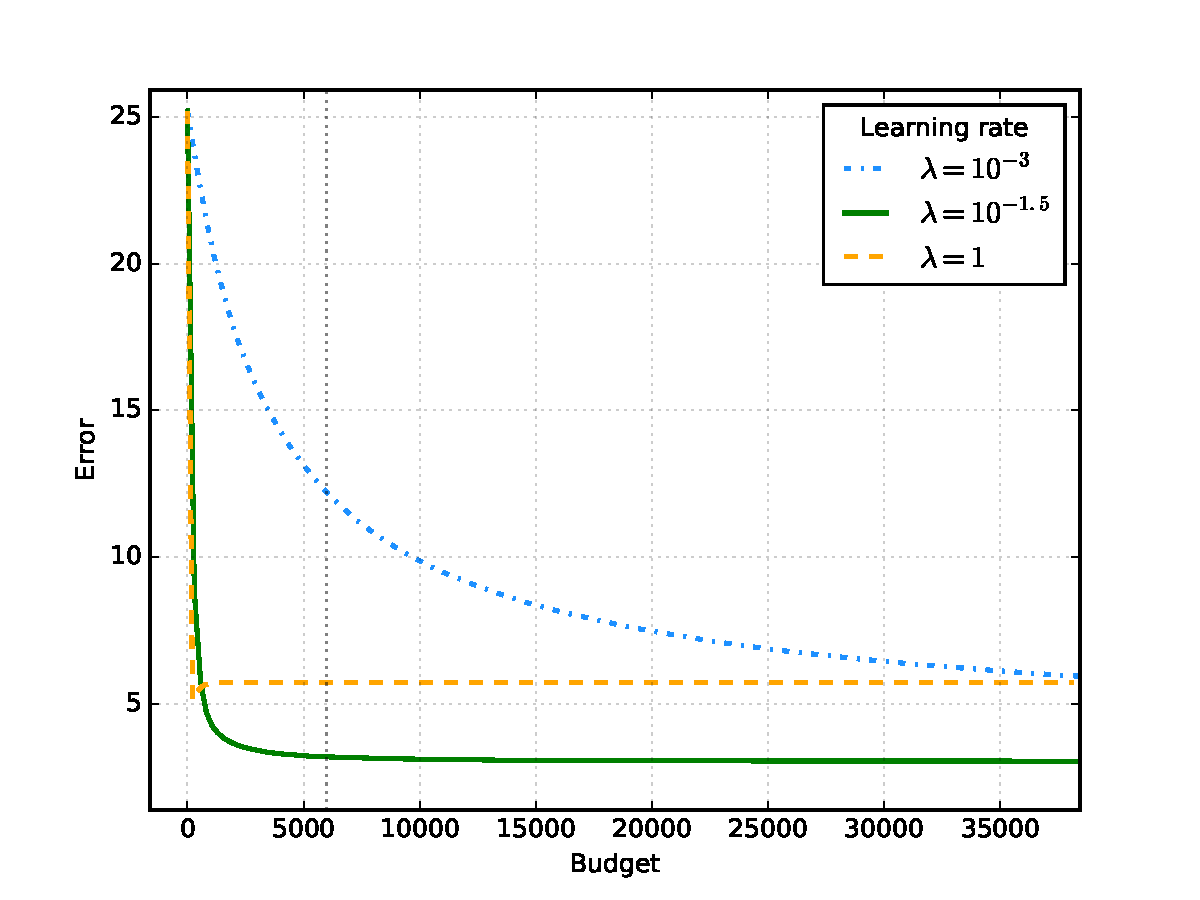
\includegraphics[width=\columnwidth]{friedman1_lr}}
\caption{Friedman1: Testing set mean square error with respect to the budget 
($CW=\infty$, m=$\sqrt{10}$, $T=1000$, budget=$59900$ ($10\%$)).}
\label{fig:learningRate}
\end{center}
\vskip -0.2in
\end{figure} 

\subsection{Influence of the hyper-parameters}
\label{subsec:hyperparams}


\paragraph{Learning rate}
Figure \ref{fig:learningRate} depicts a typical evolution of the error with the 
budget in the case of Friedman1 (the budget of $59900$ corresponds to $10\%$). 
A unit learning rate will usually decrease the test set error rapidly 
but will then either saturates or overfits. Too small a learning rate ({\it 
e.g.} $10^{-3}$) will prevent the model from reaching its minimum in the 
alloted budget.  The learning rate also influences the forest's shape, provided 
the candidate window size is large enough. On Figure \ref{fig:LRShape}, we can 
see that, for the smallest learning rate, the $80\%$ of smallest trees 
account for approximately $43\%$ of the nodes. At that stage, only $17\%$ and 
$13\%$ of the nodes are covered for the average and biggest learning rates, 
respectively. 


\begin{figure}[ht]
\begin{center}
\centerline{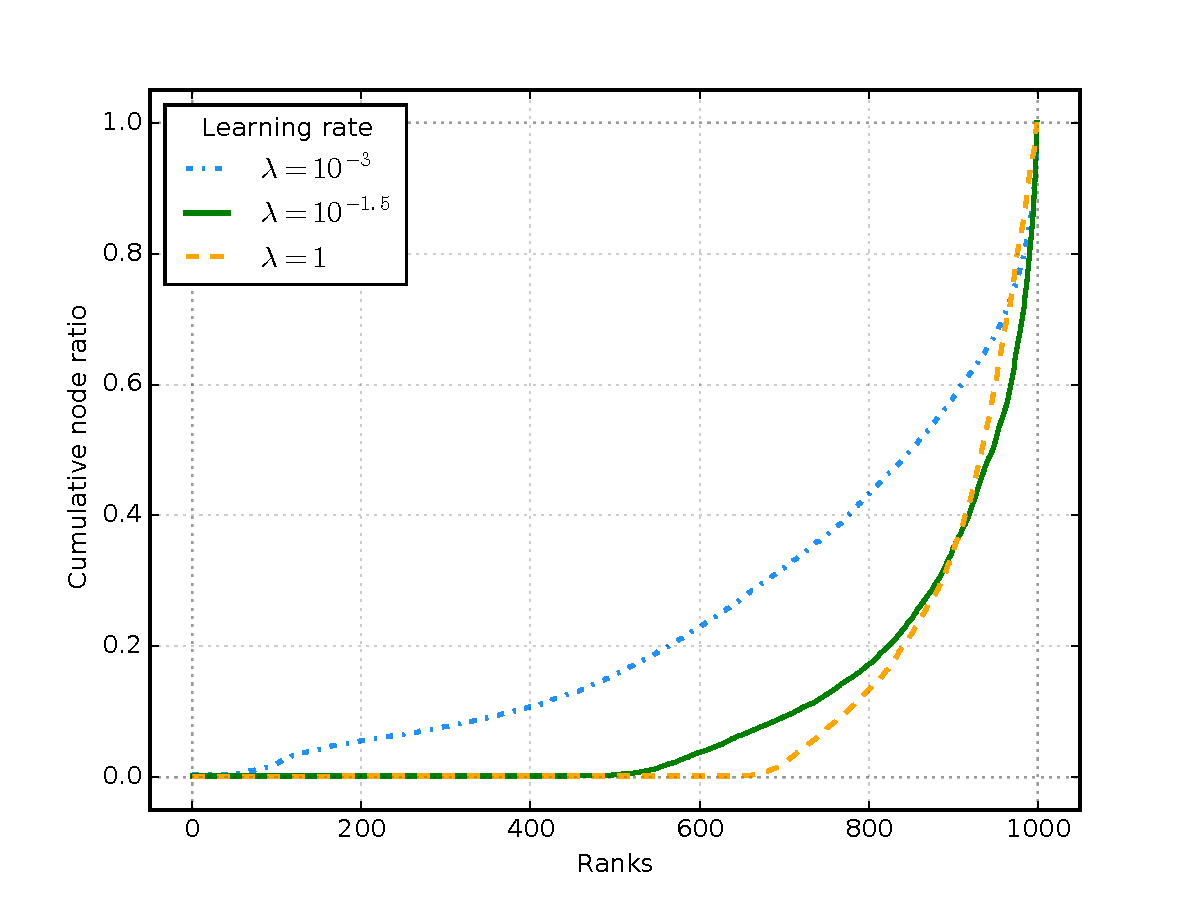
\includegraphics[width=\columnwidth]{friedman1_cumul}}
\caption{Friedman1: node distribution across tree ($CW=\infty$, 
m=$\sqrt{10}$, $T=1000$, budget=$59900$ ($10\%$)).}
\label{fig:LRShape}
\end{center}
\vskip -0.2in
\end{figure} 

%These results are corroborated by Table \ref{tab:friedEntropy}, which holds 
%the 
%entropies of the node distribution across trees. Note that entropy has been 
%normalized so that it max out at $1$.
%
%\begin{table}[t]
%\caption{Friedman1: average normalized entropy of the node distribution across 
%trees. ($CW=\infty$, m=$\sqrt{10}$, $T=1000$, budget=$59900$ ($10\%$)).}
%\label{tab:friedEntropy}
%\vskip 0.15in
%\begin{center}
%\begin{small}
%\begin{tabular}{l|ccccccc}
%\hline
%$\lambda$ & $10^{-3}$ &  $10^{-2.5}$ & $10^{-2}$ & $10^{-1.5}$ & $10^{-1}$ & 
%$10^{-0.5}$ & 1 \\
%\hline
% & 0.94 & 0.92 & 0.90 & 0.87 & 0.85 & 0.84 & 0.84
%\end{tabular}
%\end{small}
%\end{center}
%\vskip -0.1in
%\end{table}



\begin{table}[t]
\caption{Average mean square error with respect the number of 
featuer $m$ and the learning rate $\lambda$ ($CW=1$, $T=1000$, budget=$10\%$). 
In bold is $m=\sqrt{p}$.}
\label{tab:maxFeat}
\vskip 0.15in
\begin{center}
\begin{small}
CT slice
\begin{tabular}{l|ccccc}
\hline
m $\backslash$ $\lambda$  &  $10^{-2.5}$ & $10^{-2}$ & $10^{-1.5}$ & 
$10^{-1}$ & $10^{-0.5}$ \\
%\hline
%friedman
%1 & \cellcolor[gray]{0.54} 5.35 & \cellcolor[gray]{0.85} 3.35 & 
%\cellcolor[gray]{0.89} 3.05 & \cellcolor[gray]{0.87} 3.21 & 
%\cellcolor[gray]{0.78} 3.79 & \cellcolor[gray]{0.43} 6.07 \\
%{\bf 3} & \cellcolor[gray]{0.81} 3.60 & \cellcolor[gray]{0.96} 2.65 & 
%\cellcolor[gray]{1.00} 2.37 & \cellcolor[gray]{1.00} 2.39 & 
%\cellcolor[gray]{0.94} 2.75 & \cellcolor[gray]{0.68} 4.43 \\
%5 & \cellcolor[gray]{0.79} 3.76 & \cellcolor[gray]{0.92} 2.89 & 
%\cellcolor[gray]{0.97} 2.54 & \cellcolor[gray]{0.98} 2.48 & 
%\cellcolor[gray]{0.94} 2.76 & \cellcolor[gray]{0.72} 4.18 \\
%7 & \cellcolor[gray]{0.73} 4.13 & \cellcolor[gray]{0.84} 3.37 & 
%\cellcolor[gray]{0.89} 3.06 & \cellcolor[gray]{0.90} 3.03 & 
%\cellcolor[gray]{0.85} 3.34 & \cellcolor[gray]{0.63} 4.75 \\
%10 & \cellcolor[gray]{0.65} 4.63 & \cellcolor[gray]{0.74} 4.02 & 
%\cellcolor[gray]{0.77} 3.88 & \cellcolor[gray]{0.74} 4.06 & 
%\cellcolor[gray]{0.66} 4.59 & \cellcolor[gray]{0.40} 6.25 \\
\hline
{\bf 19} & \cellcolor[gray]{0.59} 27.28 & \cellcolor[gray]{0.92} 20.34 & 
\cellcolor[gray]{0.97} 19.31 & \cellcolor[gray]{0.84} 21.97 & 
\cellcolor[gray]{0.47} 29.82 \\
38 & \cellcolor[gray]{0.66} 25.78 & \cellcolor[gray]{0.96} 19.51 & 
\cellcolor[gray]{1.00} 18.63 & \cellcolor[gray]{0.89} 20.88 & 
\cellcolor[gray]{0.58} 27.62 \\
96 & \cellcolor[gray]{0.68} 25.53 & \cellcolor[gray]{0.95} 19.74 & 
\cellcolor[gray]{0.99} 18.79 & \cellcolor[gray]{0.90} 20.68 & 
\cellcolor[gray]{0.62} 26.64 \\
192 & \cellcolor[gray]{0.63} 26.55 & \cellcolor[gray]{0.89} 20.96 & 
\cellcolor[gray]{0.94} 19.92 & \cellcolor[gray]{0.86} 21.62 & 
\cellcolor[gray]{0.61} 26.87 \\
288 & \cellcolor[gray]{0.55} 28.20 & \cellcolor[gray]{0.82} 22.43 & 
\cellcolor[gray]{0.89} 20.91 & \cellcolor[gray]{0.83} 22.31 & 
\cellcolor[gray]{0.58} 27.64 \\
385 & \cellcolor[gray]{0.40} 31.42 & \cellcolor[gray]{0.70} 25.04 & 
\cellcolor[gray]{0.79} 23.11 & \cellcolor[gray]{0.74} 24.17 & 
\cellcolor[gray]{0.49} 29.56 \\
\hline
\end{tabular}
\par
Musk2\\
\begin{tabular}{l|ccccc}
\hline
m $\backslash$ $\lambda$  &  $10^{-2.5}$ & $10^{-2}$ & $10^{-1.5}$ & 
$10^{-1}$ & $10^{-0.5}$ \\
\hline
{\bf 12} & \cellcolor[gray]{0.40} 5.13 & \cellcolor[gray]{0.75} 3.74 & 
\cellcolor[gray]{0.90} 3.14 & \cellcolor[gray]{0.96} 2.90 & 
\cellcolor[gray]{0.97} 2.86 \\
16 & \cellcolor[gray]{0.43} 5.00 & \cellcolor[gray]{0.77} 3.67 & 
\cellcolor[gray]{0.91} 3.11 & \cellcolor[gray]{0.96} 2.91 & 
\cellcolor[gray]{0.97} 2.85 \\
41 & \cellcolor[gray]{0.56} 4.50 & \cellcolor[gray]{0.84} 3.39 & 
\cellcolor[gray]{0.94} 3.00 & \cellcolor[gray]{0.95} 2.93 & 
\cellcolor[gray]{0.96} 2.93 \\
83 & \cellcolor[gray]{0.62} 4.24 & \cellcolor[gray]{0.87} 3.26 & 
\cellcolor[gray]{0.96} 2.92 & \cellcolor[gray]{0.97} 2.88 & 
\cellcolor[gray]{0.96} 2.90 \\
124 & \cellcolor[gray]{0.66} 4.11 & \cellcolor[gray]{0.89} 3.20 & 
\cellcolor[gray]{0.96} 2.89 & \cellcolor[gray]{0.99} 2.79 & 
\cellcolor[gray]{1.00} 2.75 \\
166 & \cellcolor[gray]{0.66} 4.11 & \cellcolor[gray]{0.89} 3.19 & 
\cellcolor[gray]{0.95} 2.94 & \cellcolor[gray]{0.98} 2.84 & 
\cellcolor[gray]{0.97} 2.86 \\
\hline
\end{tabular}
\end{small}
\end{center}
\vskip -0.1in
\end{table}

\paragraph{Number of features}
Table \ref{tab:maxFeat} shows how the error varies with respect to both the 
learning rate and the number of features examined for a split in the case of CT 
slice and Musk2, two datasets with many features. 
Interestingly, the error tends to vary continuously over those two parameters. 
When there is more than one local minima, it is not far from the global one. 
This makes for an easy joint optimization of those two parameters. 
On both datasets, it also appears that the choice of learning rate (global 
parameter) is more critical than the number of features (local parameter). The 
optimal number of features remains problem-dependent, though. 
%Not much of a conclusion..




\begin{figure}[ht]
\begin{center}
\centerline{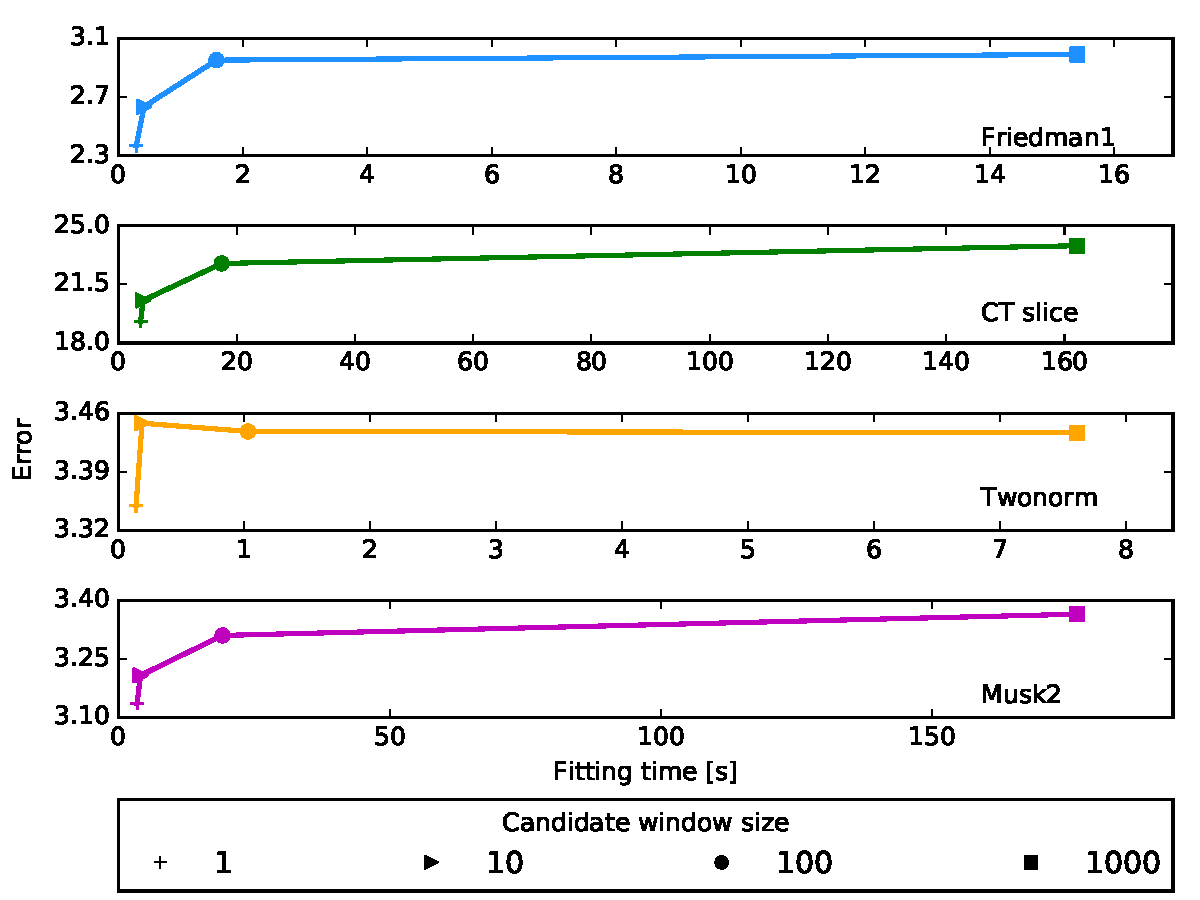
\includegraphics[width=\columnwidth]{cw_4}}
\caption{Test set error with respect to time for several values of candidate 
window size (m=$\sqrt{p}$, $T=1000$, budget=$10\%$). Friedman1 and CT slice 
were computed with the square loss and the error is mean square error. Twonorm 
and Musk2 were computed using the trimmed exponential loss with a saturation of 
$3$ and the error is the misclassification rate (in percent). Results were 
aggregated over ten runs.}
\label{fig:cw4}
\end{center}
\vskip -0.2in
\end{figure} 

\paragraph{Candidate window size}
Figure \ref{fig:cw4} illustrates the influence of the candidate window size on 
both the error and the fitting time. Firstly, the linear dependence of the 
window size on the building time is clearly visible. More interestingly, the 
smaller window size performs best on all four datasets. All in all, this seems 
to be a good regularization mechanism, allowing for a dramatic decrease of 
computation times while allowing for better predictions.

Although this is representative of the regression and binary classification, 
this is not exactly the case of multiclassification, as Table \ref{tab:cwMulti} 
shows.

\begin{table}[t]
\caption{Average misclassification rate (in percent) for the trimmed 
exponential with a saturation of $3$ (m=$\sqrt{10}$, $T=1000$, budget=$10\%$)}
\label{tab:cwMulti}
\vskip 0.15in
\begin{center}
\begin{small}
\begin{sc}
\begin{tabular}{l|cc}
\hline
Dataset & CW=$1$ & CW=$10$ \\
\hline
Waveform & 14.51 $\pm$ 0.67 & \bestA 14.05 $\pm$ 0.82 \\
Vowel & 15.90 $\pm$ 1.35 & \bestA 10.87 $\pm$ 1.61 \\
Mnist & 4.05 $\pm$ 0.25 & \bestA 3.66 $\pm$ 0.31 \\
Letter & 9.07 $\pm$ 0.53 & \bestA 5.88 $\pm$ 0.32 \\
\hline
\end{tabular}
\end{sc}
\end{small}
\end{center}
\vskip -0.1in
\end{table}



\begin{table}[t]
\caption{Average error on Friedman1 and Twonorm (trimmed exponential loss with 
saturation of $3$.) with respect to the initial number of trees $T$
($m=\sqrt{p}$, $\lambda=10^{-1.5}$, budget=$10\%$)}
\label{tab:poolsizeError}
\vskip 0.15in
\begin{center}
\begin{small}
Friedman1\\
\begin{tabular}{l|cc}
\hline
T & CW=$1$ & CW=$\infty$ \\
\hline
10 & 7.88 $\pm$ 0.64 & 7.62 $\pm$ 0.71 \\
100 & 3.31 $\pm$ 0.41 & 3.60 $\pm$ 0.35 \\
1000 & 2.37 $\pm$ 0.24 & 3.05 $\pm$ 0.29 \\
10000 & 2.26 $\pm$ 0.20 & 3.18 $\pm$ 0.28 \\
\hline
\end{tabular}
\par
Twonorm \\
\begin{tabular}{c|cc}
\hline
T & CW=$1$ & CW=$\infty$ \\
\hline
10 & 7.47 $\pm$ 0.73 & 7.05 $\pm$ 0.29 \\
100 & 3.44 $\pm$ 0.16 & 3.52 $\pm$ 0.13 \\
1000 & 3.35 $\pm$ 0.22 & 3.43 $\pm$ 0.23 \\
10000 & 3.53 $\pm$ 0.25 & 3.87 $\pm$ 0.32 \\
\hline
\end{tabular}
\end{small}
\end{center}
\vskip -0.1in
\end{table}


\begin{table}[t]
\caption{Friedman1: average normalized node distribution across trees' entropy 
on Friedman1 
%and Twonorm (trimmed exponential loss with saturation of $3$.) 
with respect to the initial number of trees $T$ ($m=\sqrt{p}$, 
$\lambda=10^{-1.5}$, budget=$10\%$)}
\label{tab:poolsizeEntropy}
\vskip 0.15in
\begin{center}
\begin{small}
%Friedman1\\
\begin{tabular}{c|c|ccc}
\hline
 & CW=$1$ & \multicolumn{3}{c}{CW=$\infty$} \\
T $\backslash$ $\lambda$ & * & $10^{-3}$ & $10^{-1.5}$ & $1$ \\
\hline
%10 & 100.00 & 100.00 & 100.00 & 99.93 \\
100 & 99.89 & 99.84 & 99.24 & 98.48 \\
1000 & 98.15 & 94.49 & 87.32 & 83.72 \\
10000 & 97.20 & 89.12 & 76.23 & 68.99 \\
\hline
\end{tabular}
%\par
%Twonorm \\
%\begin{tabular}{c|c|ccc}
%\hline
% & CW=$1$ & \multicolumn{3}{c}{CW=$\infty$} \\
%T $\backslash$ $\lambda$ & $10^{-1.5}$ & $10^{-3}$ & $10^{-1.5}$ & $1$ \\
%\hline
%10 & 99.85 & 99.85 & 99.88 & 99.90 \\
%100 & 99.93 & 99.92 & 99.91 & 99.93 \\
%1000 & 97.90 & 96.99 & 91.55 & 91.78 \\
%10000 & 93.31 & 87.08 & 83.48 & 79.99 \\
%\hline
%\end{tabular}
\end{small}
\end{center}
\vskip -0.1in
\end{table}

\begin{table}[t]
\caption{Average fitting time (in seconds) on Friedman1 with respect to the 
initial number of trees $T$ ($m=\sqrt{p}$, $\lambda=10^{-1.5}$, budget=$10\%$)}
\label{tab:poolsizeTime}
\vskip 0.15in
\begin{center}
\begin{small}
\begin{tabular}{c|c|cc}
\hline
 & CW=$1$ & \multicolumn{2}{c}{CW=$\infty$} \\
T $\backslash$ $\lambda$ & * & $10^{-3}$ &  $1$ \\
\hline
100 & 0.34 $\pm$ 0.07 & 0.35 $\pm$ 0.07 &  0.32 $\pm$ 0.07 \\
1000 & 0.59 $\pm$ 0.12 & 3.84 $\pm$ 0.18 & 2.78 $\pm$ 0.54 \\
10000 & 1.55 $\pm$ 0.02 & 25.95 $\pm$ 1.05 & 20.69 $\pm$ 
2.92 \\
\hline
\end{tabular}
\end{small}
\end{center}
\vskip -0.1in
\end{table}

\paragraph{Number of trees}
The initial number of trees is an intricate parameter, as its impacts the 
model's predictions, the fitting time and the shape of the forest.

Table \ref{tab:poolsizeError} focuses on the errors. Unsurprisingly, the models 
perform badly when it has only 10 trees as its disposal; this leaves only few 
room for the learning algorithm to optimize globally. The more tree is not 
always the better, however. When the candidate window is infinitely large, this 
might be due to overfitting: there are so many candidates to choose from that 
over-optimization hurts the model. When the window size is $1$, this is more 
directly linked to the forest's shape.

Table \ref{tab:poolsizeEntropy} holds the normalized entropy of the node 
distribution across trees. By ``normalized'', we mean that the entropy was 
divided by $\log_2 T$ and then multiplied by $100$.
Only one value is reported for the case $CW=1$ as the forest has always the 
same shape. The evolution of the entropy for a fix number of trees when 
$CW=\infty$ has already been commented on. It is rendered more obvious when the 
initial number of trees is larger, however, meaning that GIF is able to exploit 
the greater freedom offered by the additional trees. 
When $CW=1$, the distribution is much closer to being uniform (entropy 
close to $100$) than when the learning algorithm can adapt the forest's shape. 
If this shapes does not agree with the data, the model might perform less well. 
Nevertheless, as we saw, $CW=1$ yield better result on all but the multiclass 
problems, and $T=1000$ seems to be adequate in average. %Poor way to conclude

The number of trees also impacts the learning time, as depicted by Table 
\ref{tab:poolsizeTime}. The linear increase in computation time in the case of 
$CW=\infty$ is due to the global optimization of the chosen node that must run 
through all the candidates. In the case of $CW=1$, the computation time is 
almost not burdened by the number of trees. The slight increase is actually 
related to the forest's shape: since the distribution of node tends to be more 
uniform, the algorithm must run through more examples while optimizing the 
weights (higher part of the trees).


\subsection{Comparison with Boosting}
\label{subsec:boosting}

\begin{table}[t]
\caption{Average error for Boosting.}
\label{tab:boosting}
\vskip 0.15in
\begin{center}
\begin{small}
\begin{sc}
\begin{tabular}{l|c|c}
\hline
Datasets & $10\%$ & $1\%$ \\
\hline
Friedman1 & 4.53 $\pm$ 0.23 & 3.86 $\pm$ 0.10 \\
Abalone & 5.17 $\pm$ 0.20 & 4.83 $\pm$ 0.20 \\
CT slice & 82.44 $\pm$ 3.80 & 68.73 $\pm$ 1.92 \\
Hwang $\times 10{-2}$ & 97.88 $\pm$ 2.33 &  88.62 $\pm$ 1.73 \\
\hline
Ringnorm & 5.48 $\pm$ 0.55 & 6.71 $\pm$ 0.99 \\
Twonorm & 5.09 $\pm$ 0.56 & 5.98 $\pm$ 0.47 \\
Hastie & 5.65 $\pm$ 0.34 & 7.10 $\pm$ 0.41 \\
Musk2 & 2.70 $\pm$ 0.37 & 4.20 $\pm$ 0.28 \\
Madelon & 11.30 $\pm$ 0.68 & 11.33 $\pm$ 0.69 \\
\hline
\end{tabular}
\end{sc}
\end{small}
\end{center}
\vskip -0.1in
\end{table}
%Hwang Depth=2 & 11.09 $\pm$ 0.25 || Depth=2 & 8.40 $\pm$ 0.19 \\


Although not our starting point, Boosting is an other method to build ensemble 
of trees. In this section, we compare how GIF fares against it. 

To submit Boosting to the budget constraint, we have used stumps as base 
learners and have made as many trees as were necessary to meet the constraint. 
We have used the same learning rate as in GIF. Regression has been tackled with 
Gradient Boosting over a square loss. Adaboost is in charge of classification. 
Therefore, the same losses are used in GIF and Boosting.
%TODO ref for Adaboost?

Table \ref{tab:boosting} holds the errors for Boosting at $1\%$ and $10\%$. In 
the default settings, GIF beats Boosting on all regression datasets but Abalone 
where it performs slightly less well. Interestingly, Boosting also overfits on 
Abalone and Hwang. The situation is more contrasted in classification, where 
Boosting outperforms GIF on Hastie and Musk2 for both budget constraints.

Notice that stumps did not agree with Hwang and CT slice, where a depth of $2$ 
would yield errors of $11.09 \pm 0.25$ and $8.40 \pm 0.19$ at $10\%$ and 
$1\%$ respectively for Hwang and $33.53 \pm 1.65$ and $36.67 \pm 1.36$ at 
$10\%$ and $1\%$ respectively for CT slice. However, this does not change the 
conclusions regarding those datasets.

Since the base learners in Boosting are shallow, both its fitting and 
prediction time are greater than GIF's ($CW=1$), as table 
\ref{tab:boostingTime} confirms.

Overall, the performances of Boosting and GIF in terms of errors are somewhat 
similar. Sometimes GIF's extra-layers of regularization, combined with a 
greater variety of depths pays off and sometimes not. However, GIF is faster in 
both learning and prediction.


\begin{table}[t]
\caption{Average fitting and prediction time (in seconds) on Musk2 for 
Boosting (depth=$1$, $\lambda=10^{-1.5}$) and GIF (trimmed exponenantial loss 
with saturation=3, $T=1000$ $m=\sqrt{p}$, $\lambda=10^{-1.5}$) for a budget of 
$10\%$.}
\label{tab:boostingTime}
\vskip 0.15in
\begin{center}
\begin{small}
\begin{tabular}{l|c|c}
\hline
& Boosting & GIF \\
\hline
Fitting & 399.17 $\pm$ 60.91 & 1.53 $\pm$ 0.04 \\
Prediction & 28.39 $\pm$ 5.43 & 0.31 $\pm$ 0.07 \\
\hline
\end{tabular}
\end{small}
\end{center}
\vskip -0.1in
\end{table}



%\subsection{Comparison with post-pruning}





\section{Conclusion and perspectives}
\label{sec:conclusion}

In this paper, we introduced the Globally Induced Forest (GIF) whose goal is to 
produce lightweight yet accurate models by sequentially adding nodes to the 
model. Contrary to most tree-aware techniques, our method does not require the 
{\it a priori} building of the whole forest and works on the whole learning set.

Although starting from the Random forest perspective, the learning algorithm 
shares similar traits with Boosting, the main differences being the extra layer 
of regularization and the shape adaptability of GIF.

Several hyper-parameters govern the learning algorithm. We have proposed a set 
of default parameters which seems to work quite well in average, beating, under 
mild and severe memory constraints, both the Extremely randomized trees and 
Boosting on several datasets. Needless to say that the setting can be further 
refined if necessary.

Of the most interest is that it is usually better no to optimize the choice of 
nodes. In other words, letting the algorithm optimize the forest's shape 
is---surprisingly---harmful. Although it complicates the choice of the 
initial number of trees, this makes for an incredibly fast learning algorithm.

Sadly, and despite proposing an elegant scheme for multiclass problems, GIF 
seems to run into troubles with them. This should be the main focus of 
subsequent works.

The quality of the variable importance measures have not been examined, nor the 
ability of the forest to serve as codebook, two frequent uses of the tree-based 
techniques. Aside from that, several extensions can be thought of. For 
instance, one could allow for the refitting of the already chosen nodes by 
leaving them in the candidate list. The split might also be optimized globally 
if the candidate window is small enough. Multi-output losses which take into 
account the correlation between the outputs can be proposed. Finally, a online 
variant of the algorithm would be interesting for the case where a extremely 
lightweight model is desired on a very large dataset.













\appendix
\section{Equivalence of GIF and the underlying tree}\label{app:Equiv}
In the case of a single tree and a unit learning rate, both the square loss in 
regression and the multiexponential loss in classification produce the same 
prediction as the underlying tree. 
This is due to the fact that, when examining the weight to give to node $j$ at 
time $t$, the prediction of time $t-1$ relates to the parent $\pi_j$ of $j$. It 
is thus independent of $t$ and is also the same for all instance reaching that 
node. Consequently, we will adopt the following slight change in notation:

\begin{align}
\hat{y}_j = \hat{y}_{(\pi_j)} + w_j
\end{align}

Meaning that the prediction associated to any object reaching node $j$ is the 
weight of $j$ plus the prediction associated to its parent $\pi_j$. With 
$\hat{y}_{(\pi_1)} = 0$, the prediction of the root's pseudo-parent.

\subsection{Regression}
In regression, the tree prediction $Tr_j$ of any leaf $j$ is the average of the 
learning set's outputs reaching that node: $Tr_j = \frac{1}{|Z_j|}\sum_{i \in 
Z_j} y_i$. We need to show that the GIF prediction is:

\begin{align}\label{eq:EquivL2Cond}
\hat{y}_{j} = \frac{1}{|Z_j|}\sum_{i \in Z_j} y_i
\end{align}


The prediction of node $j$ is

\begin{align}\label{eq:EquivL2Solution}
\hat{y}_j &= \hat{y}_{\pi_j} + w_j \\
&= \hat{y}_{\pi_j} +  \frac{1}{|Z_j|} \sum_{i \in Z_j} \left(y_i - 
\hat{y}_{\pi_j}\right) \\
&= \hat{y}_{\pi_j} + \frac{1}{|Z_j|} \sum_{i \in Z_j} \left( y_i \right) - 
\hat{y}_{\pi_j} \\
&= \frac{1}{|Z_j|} \sum_{i \in Z_j}  y_i 
\end{align}
The first step is how the additive model is built. The second is the optimal 
weight value of node $j$ derived in Equation \ref{eq:L2Solution}, the third 
step is due to the fact that the prediction at $\pi_j$ is constant since there 
is only one tree.

\subsection{Classification}
In order to have the same prediction as the underlying tree, we must 
demonstrate that the probability of being in class $l$ associated to node $j$ 
will be $\frac{Z_j^{(l)}}{|Z_j|}$.
Under the zero-sum constraint, we have

\begin{align} 
\exp \left(  \frac{1}{K-1} w_j^{(l)}\right) &= \frac{1}{c_j} 
\alpha_{\pi_i}^{(l)} \\
&=  \frac{1}{c_j} \sum_{i \in Z_j^{(l)}} \exp \left(-\frac{1}{K-1} 
\hat{y}_{\pi_i}^{(l)}\right)\\
&= |Z_j^{(l)}| \exp \left(-\frac{1}{K-1} \hat{y}_j^{(l)}\right) \\
\exp \left(\frac{1}{K-1} \hat{y}_j^{(l)} \right) &= \exp \left(\frac{1}{K-1} 
\hat{y}_{\pi_j}^{(l)} \right) \exp \left(\frac{1}{K-1} w_j^{(l)}\right) \\
&= \frac{1}{c_j} |Z_j^{(l)}| \\
P_j(l) &= \frac{\exp \left(\frac{1}{K-1} \hat{y}_j^{(l)}
\right)}{\sum_{k=1}^K\exp \left(\frac{1}{K-1} \hat{y}_j^{(k)} \right)} = 
\frac{|Z_j^{(l)}|}{|Z_j|}
\end{align}

where $c_j = \left(\prod_{k=1}^K \alpha_j^{(k)}\right)^{\frac{1}{K}}$ is a 
constant. The first equality is a consequence of the value of $w_j^{(l)}$ 
(Equation \ref{eq:MEsolution}). The second is a due to the definition of 
$\alpha_j^{(l)}$ (Equation \ref{eq:MEClsErrZS}). The third is a consequence of 
having a single tree: the prediction of the parent is the same for all 
instances.





Notice that, in both regression and classification, the equivalence also holds 
for an internal node: the prediction is the one the tree would have yielded if 
that node had been a leaf.


\bibliography{gif}
\bibliographystyle{icml2016}

\end{document} 

